\subsection{Repensar estatístico}

Muita coisa pode dar errado com a inferência estatística, e esta é uma das razões pelas quais os iniciantes ficam tão ansiosos com ela. Quando a estrutura consiste em escolher um teste pré-fabricado em um fluxograma, a ansiedade pode aumentar à medida que se teme não escolher o teste "correto". Os estatísticos, por sua vez, podem sentir prazer em repreender os cientistas, piorando a batalha psicológica.

Mas a ansiedade pode ser cultivada em sabedoria. Essa é a razão pela qual este livro insiste em trabalhar com os detalhes computacionais de cada golem. Se você não entende como o golem processa a informação, não pode interpretar a saída do golem. Isso requer conhecer o modelo estatístico em maior detalhe do que o habitual, e requer fazer os cálculos do jeito difícil, pelo menos até que você seja sábio o suficiente para usar as soluções de apertar um botão.

Existem obstáculos conceituais também, obstáculos relacionados a como os estudiosos definem os objetivos estatísticos e interpretam os resultados estatísticos. Entender qualquer golem individual não é suficiente nesses casos. Em vez disso, precisamos de alguma epistemologia estatística, uma apreciação de como os modelos estatísticos se relacionam com as hipóteses e com os mecanismos naturais de interesse. Afinal, o que se supõe que estejamos fazendo com essas pequenas máquinas computacionais?

O maior obstáculo que encontro entre alunos e colegas é a crença tácita de que o objetivo adequado da inferência estatística é testar hipóteses nulas. Este é o objetivo correto, diz o pensamento, porque Karl Popper argumentou que a ciência avança ao falsificar hipóteses. Karl Popper (1902–1994) é possivelmente o filósofo da ciência mais influente, pelo menos entre os cientistas. Ele argumentou persuasivamente que a ciência funciona melhor ao desenvolver hipóteses que são, em princípio, falsificáveis. Buscar evidências que possam embaraçar nossas ideias é um padrão normativo, e ao qual a maioria dos estudiosos — quer se descrevam como cientistas ou não — adere. Então, talvez os procedimentos estatísticos devessem falsificar hipóteses, se desejamos ser bons cientistas estatísticos.

Mas o que foi dito acima é um tipo de Popperismo folclórico, uma filosofia informal da ciência comum entre cientistas, mas não entre filósofos da ciência. A ciência não é descrita pelo padrão de falsificação, e Popper reconheceu isso. De fato, a falsificação dedutiva é impossível em quase todos os contextos científicos. Nesta seção, reviso duas razões para essa impossibilidade.

\begin{enumerate}
  \item \textbf{Hipóteses não são modelos.} As relações entre hipóteses e diferentes tipos de modelos são complexas. Muitos modelos correspondem à mesma hipótese, e muitas hipóteses correspondem a um único modelo. Isso torna a falsificação estrita impossível.
  \item \textbf{A medição importa.} Mesmo quando pensamos que os dados falsificam um modelo, outro observador debaterá nossos métodos e medidas. Eles não confiam nos dados. Às vezes, eles estão certos.
\end{enumerate}

Por ambas as razões, a falsificação dedutiva nunca funciona. O método científico não pode ser reduzido a um procedimento estatístico, e por isso nossos métodos estatísticos não devem fingir que podem. A evidência estatística é parte da grande bagunça que é a ciência, com todo o seu combate, egotismo e coerção mútua. Se você acredita, como eu, que a ciência muitas vezes funciona, então aprender que ela não funciona por meio da falsificação não deve mudar sua opinião. Mas pode ajudá-lo a fazer ciência melhor, pois abrirá seus olhos para muitas funções legitimamente úteis dos golems estatísticos.

\begin{quote}
  \textbf{Repensando: O NHST é falsificacionista?} O teste de significância de hipótese nula, NHST (\textit{Null hypothesis significance testing}), é frequentemente identificado com a filosofia da ciência falsificacionista, ou Popperiana. No entanto, geralmente o NHST é usado para falsificar uma hipótese nula, não a hipótese de pesquisa real. Portanto, a falsificação está sendo feita em algo diferente do modelo explicativo. Isso parece o inverso da filosofia de Karl Popper.
\end{quote}

\subsubsection{Hipóteses não são modelos}

Quando tentamos falsificar uma hipótese, devemos trabalhar com um modelo de algum tipo. Mesmo quando a tentativa não é explicitamente estatística, há sempre um modelo tácito de medição, de evidência, que operacionaliza a hipótese. Todos os modelos são falsos, então o que significa falsificar um modelo? Uma consequência da exigência de trabalhar com modelos é que não é mais possível deduzir que uma hipótese é falsa, apenas porque rejeitamos um modelo derivado dela.

Vamos explorar essa consequência no contexto de um exemplo da biologia populacional (FIGURA 1.2). Começando na década de 1960, biólogos evolucionistas se interessaram pela proposta de que a maioria das mudanças evolutivas na frequência gênica é causada não pela seleção natural, mas sim por mutação e deriva. Ninguém realmente duvidava que a seleção natural fosse responsável pelo design funcional. Este era um debate sobre sequências genéticas. Assim começaram várias décadas produtivas de combate acadêmico sobre modelos "neutros" de evolução molecular. Esse combate está mais fortemente associado a Motoo Kimura (1924–1994), que talvez tenha sido o mais forte defensor dos modelos neutros. Mas muitos outros geneticistas de populações participaram. Com o passar do tempo, disciplinas relacionadas como ecologia de comunidades e antropologia experimentaram (ou estão experimentando atualmente) suas próprias versões do debate da neutralidade.

Vamos usar o esquema na FIGURA 1.2 para explorar conexões entre hipóteses motivadoras e diferentes modelos, no contexto do debate da evolução neutra. À esquerda, há duas hipóteses estereotipadas e informais: Ou a evolução é "neutra" ($H_0$) ou a seleção natural importa de alguma forma ($H_1$). Essas hipóteses têm limites vagos, porque começam como conjecturas verbais, não modelos precisos. Existem milhares de processos detalhados possíveis que podem ser descritos como "neutros", dependendo das escolhas sobre, por exemplo, estrutura populacional, número de locais, número de alelos em cada local, taxas de mutação e recombinação.

Uma vez feitas essas escolhas, temos a coluna do meio na FIGURA 1.2, os \textsc{modelos de processo} detalhados de evolução. $P_{0A}$ e $P_{0B}$ diferem no fato de que um assume que o tamanho e a estrutura da população têm sido constantes por tempo suficiente para que a distribuição de alelos atinja um estado estacionário. O outro imagina, em vez disso, que o tamanho da população flutua ao longo do tempo, o que pode ser verdade mesmo quando não há diferença seletiva entre os alelos. A hipótese "a seleção importa" $H_1$ da mesma forma corresponde a muitos modelos de processo diferentes. Mostrei dois grandes protagonistas: um modelo no qual a seleção sempre favorece certos alelos e outro no qual a seleção flutua ao longo do tempo, favorecendo diferentes alelos.

Uma característica importante desses modelos de processo é que eles expressam uma estrutura causal. Diferentes modelos de processo formalizam diferentes relações de causa e efeito. Quer analisada matematicamente ou por simulação, a direção do tempo em um modelo significa que algumas coisas causam outras, mas não o inverso. Você pode usar tais modelos para realizar experimentos e investigar suas implicações causais. Às vezes, essas investigações revelam, antes mesmo de passarmos para a inferência estatística, que o modelo não pode explicar um fenômeno de interesse.

% INSERIR A FIGURA 1.2 AQUI
\begin{figure}[htbp]
  \centering
  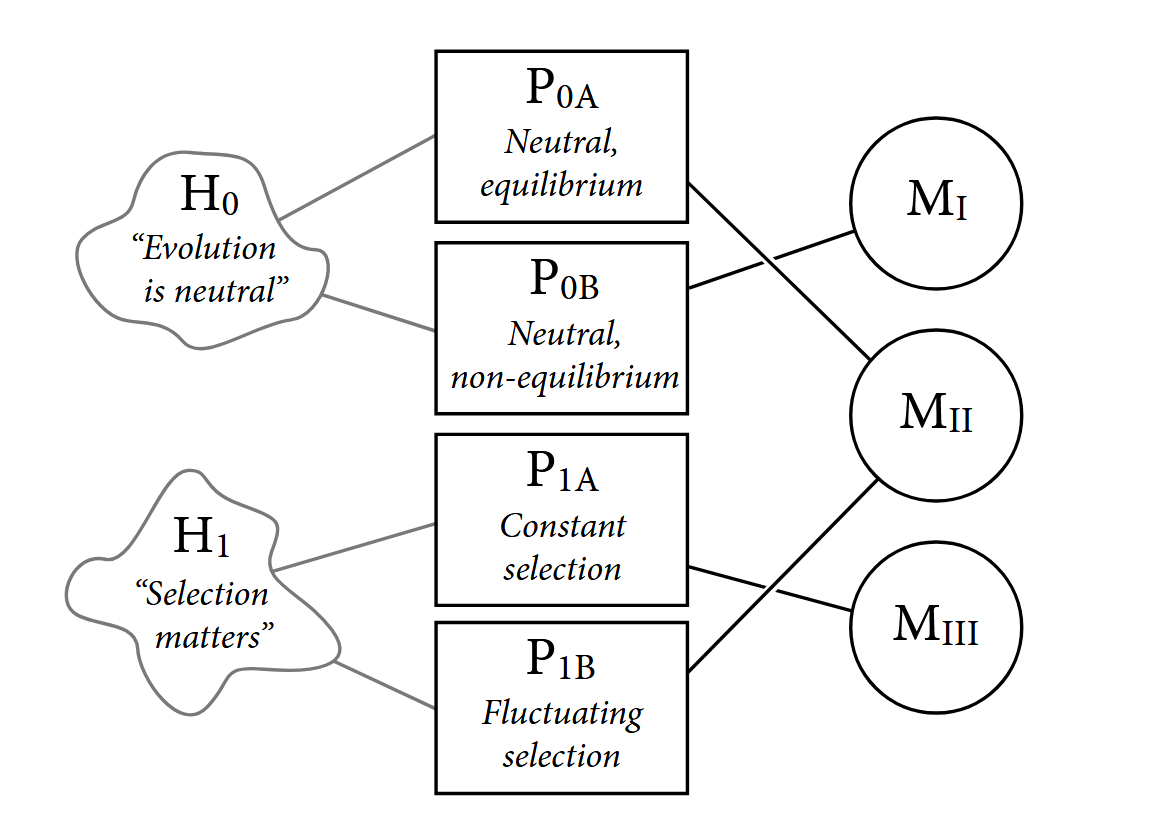
\includegraphics[width=\textwidth]{img/fig1_2.png}
  \caption{Relações entre hipóteses (esquerda), modelos de processo detalhados (meio) e modelos estatísticos (direita), ilustrados pelo exemplo de modelos "neutros" de evolução. As hipóteses ($H$) são tipicamente vagas e, portanto, correspondem a mais de um modelo de processo ($P$). As avaliações estatísticas de hipóteses raramente abordam os modelos de processo diretamente. Em vez disso, elas dependem de modelos estatísticos ($M$), os quais refletem apenas alguns aspectos dos modelos de processo. Como resultado, as relações são múltiplas em ambas as direções: Hipóteses não implicam modelos únicos, e modelos não implicam hipóteses únicas. Esse fato complica enormemente a inferência estatística.}
  \label{fig:1.2}
\end{figure}

Para desafiar os modelos de processo com dados, eles precisam ser transformados em modelos estatísticos. Infelizmente, os modelos estatísticos não incorporam relações causais específicas. Um modelo estatístico expressa associações entre variáveis. Como resultado, muitos modelos de processo diferentes podem ser consistentes com qualquer modelo estatístico único.

Como obtemos um modelo estatístico a partir de um modelo causal? Uma maneira é derivar a distribuição de frequência esperada de alguma quantidade — uma "estatística" — a partir do modelo causal. Por exemplo, uma estatística comum neste contexto é a distribuição de frequência (histograma) da frequência de diferentes variantes genéticas (alelos). Alguns alelos são raros, aparecendo em apenas alguns indivíduos. Outros são muito comuns, aparecendo em muitos indivíduos na população. Um resultado famoso na genética de populações é que um modelo como $P_{0A}$ produz uma distribuição de \textit{lei de potência} das frequências alélicas. E assim esse fato produz um modelo estatístico, $M_{II}$, que prevê uma lei de potência nos dados. Em contraste, o modelo de processo de seleção constante $P_{1A}$ prevê algo bem diferente, $M_{III}$.

Infelizmente, outros modelos de seleção ($P_{1B}$) implicam o mesmo modelo estatístico, $M_{II}$, que o modelo neutro. Eles também produzem leis de potência. Então chegamos à lição desconfortável:

\begin{enumerate}
  \item Qualquer modelo estatístico ($M$) dado pode corresponder a mais de um modelo de processo ($P$).
  \item Qualquer hipótese ($H$) dada pode corresponder a mais de um modelo de processo ($P$).
  \item Qualquer modelo estatístico ($M$) dado pode corresponder a mais de uma hipótese ($H$).
\end{enumerate}

Agora veja o que acontece quando comparamos os modelos estatísticos aos dados. A abordagem clássica é tomar o modelo "neutro" como uma hipótese nula. Se os dados não forem suficientemente semelhantes à expectativa sob a nula, então dizemos que "rejeitamos" a hipótese nula. Suponha que sigamos o histórico deste assunto e tomemos $P_{0A}$ como nossa hipótese nula. Isso implica dados correspondentes a $M_{II}$. Mas como o mesmo modelo estatístico corresponde a um modelo de seleção $P_{1B}$, não está nem um pouco claro o que devemos fazer em relação a rejeitar ou aceitar a nula. O modelo nulo não é único para nenhum modelo de processo nem hipótese. Se rejeitarmos a nula, não podemos realmente concluir que a seleção importa, porque existem outros modelos neutros que preveem distribuições diferentes de alelos. E se falharmos em rejeitar a nula, não podemos realmente concluir que a evolução é neutra, porque alguns modelos de seleção esperam a mesma distribuição de frequência.

Este é um grande incômodo. Uma vez que temos o diagrama na FIGURA 1.2, é fácil ver o problema. Mas poucos de nós têm tanta sorte. Enquanto a genética de populações reconheceu esse problema, acadêmicos em outras disciplinas continuam a testar distribuições de frequência contra as expectativas da lei de potência, argumentando até mesmo que existe apenas um modelo neutro. Mesmo que houvesse apenas um modelo neutro, existem tantos modelos não neutros que imitam as previsões da neutralidade, que nem rejeitar nem falhar em rejeitar o modelo nulo carrega muito poder inferencial.

Então o que pode ser feito? Bem, se você tem múltiplos modelos de processo, muita coisa pode ser feita. Se acontece que todos os modelos de processo de interesse fazem previsões muito semelhantes, então você sabe que deve procurar uma descrição diferente da evidência, uma descrição sob a qual os processos pareçam diferentes. Por exemplo, embora $P_{0A}$ e $P_{1B}$ façam previsões de lei de potência muito semelhantes para a distribuição de frequência de alelos, eles fazem previsões muito diferentes para a distribuição de mudanças na frequência alélica ao longo do tempo. Compare explicitamente as previsões de mais de um modelo e você pode se salvar de alguns tipos comuns de loucura.

Os modelos estatísticos também podem ser confundidos de outras maneiras, como a confusão causada por variáveis não observadas e viés de amostragem. Modelos de processo nos permitem projetar modelos estatísticos com esses problemas em mente. O modelo estatístico por si só não é suficiente.

\begin{quote}
  \textbf{Repensando: Entropia e identificação do modelo.} Uma razão pela qual os modelos estatísticos correspondem rotineiramente a muitos modelos de processo detalhados diferentes é porque eles dependem de distribuições como a normal, binomial, Poisson e outras. Essas distribuições são membros de uma família, a \textsc{família exponencial}. A natureza ama os membros desta família. A natureza os ama porque a natureza ama a entropia, e todas as distribuições da família exponencial são distribuições de \textsc{entropia máxima}. Tirar a personificação natural dessa explicação terá que esperar até o Capítulo 10. A implicação prática é que não se pode inferir o processo evolutivo a partir de uma lei de potência mais do que se pode inferir o processo de desenvolvimento a partir do fato de que a altura é normalmente distribuída. Esse fato deve nos tornar humildes sobre o que modelos típicos de regressão — o cerne deste livro — podem nos ensinar sobre processos mecanísticos. Por outro lado, a natureza de entropia máxima dessas distribuições significa que podemos usá-las para fazer trabalho estatístico útil, mesmo quando não conseguimos identificar o processo subjacente. Não apenas não podemos identificá-lo, mas também não precisamos.
\end{quote}

\subsubsection{A medição importa}

A lógica da falsificação é muito simples. Temos uma hipótese $H$, e mostramos que ela implica alguma observação $D$. Então procuramos por $D$. Se não a encontrarmos, devemos concluir que $H$ é falsa. Os lógicos chamam esse tipo de raciocínio de \textit{modus tollens}, que é uma abreviação em latim para "o método de destruição". Em contraste, encontrar $D$ não nos diz nada certo sobre $H$, porque outras hipóteses também podem prever $D$.

Uma fábula científica convincente que emprega o \textit{modus tollens} diz respeito à cor dos cisnes. Antes de descobrir a Austrália, todos os cisnes que qualquer europeu já tinha visto tinham penas brancas. Isso levou à crença de que todos os cisnes são brancos. Vamos chamar isso de uma hipótese formal:
$$H_0: \text{Todos os cisnes são brancos.}$$

Quando os europeus chegaram à Austrália, no entanto, eles encontraram cisnes com penas pretas. Essa evidência pareceu provar instantaneamente que $H_0$ era falsa. De fato, nem todos os cisnes são brancos. Alguns são certamente pretos, de acordo com todos os observadores. A principal percepção aqui é que, antes de viajar para a Austrália, nenhum número de observações de cisnes brancos poderia provar que $H_0$ era verdadeira. No entanto, exigiu-se apenas uma observação de um cisne negro para provar que era falsa.

Esta é uma história sedutora. Se podemos acreditar que hipóteses científicas importantes podem ser declaradas desta forma, então temos um método poderoso para melhorar a precisão de nossas teorias: procurar evidências que desconfirmem nossas hipóteses. Sempre que encontramos um cisne negro, $H_0$ deve ser falsa. Progresso!

Buscar evidências desconfirmadoras é importante, mas não pode ser tão poderoso quanto a história do cisne faz parecer. Além dos problemas de correspondência entre hipóteses e modelos, discutidos na seção anterior, a maioria dos problemas que os cientistas enfrentam não são tão logicamente discretos. Em vez disso, frequentemente enfrentamos dois problemas simultâneos que tornam a fábula do cisne não representativa. Primeiro, as observações são propensas a erros, especialmente nas fronteiras do conhecimento científico. Segundo, a maioria das hipóteses é quantitativa, referindo-se a graus de existência, em vez de discretas, referindo-se à presença ou ausência total. Vamos considerar brevemente cada um desses problemas.

\subsubsection{Erro de observação}

Todos os observadores concordarão sob a maioria das condições que um cisne é preto ou branco. Existem poucos tons intermediários, e os olhos da maioria dos observadores funcionam de maneira semelhante o suficiente para que haja pouca, se alguma, discordância sobre quais cisnes são brancos e quais são pretos. Mas esse tipo de exemplo dificilmente é comum na ciência, pelo menos em campos maduros. Em vez disso, rotineiramente confrontamos contextos em que não temos certeza se detectamos um resultado desconfirmador. Nas fronteiras do conhecimento científico, a capacidade de medir um fenômeno hipotético muitas vezes está tão em questão quanto o próprio fenômeno.

Aqui estão dois exemplos.

Em 2005, uma equipe de ornitólogos de Cornell alegou ter evidências de um indivíduo de Pica-pau-bico-de-marfim (\textit{Campephilus principalis}), uma espécie que se pensava estar extinta. A hipótese implícita aqui é:
$$H_0: \text{O Pica-pau-bico-de-marfim está extinto.}$$

Seria necessária apenas uma observação para falsificar essa hipótese. No entanto, muitos duvidaram da evidência. Apesar dos extensos esforços de busca e de uma recompensa em dinheiro de US\$ 50.000 por informações que levassem a um espécime vivo, nenhuma evidência que satisfaça a todas as partes emergiu até agora (em 2015). Mesmo que surjam boas evidências físicas eventualmente, este episódio deve servir como um contraponto à história do cisne. Encontrar casos desconfirmadores é complicado pelas dificuldades de observação. Cisnes negros nem sempre são realmente cisnes negros, e às vezes cisnes brancos são na verdade cisnes negros. Existem confirmações equivocadas (falsos positivos) e desconfirmações equivocadas (falsos negativos). Contra esse pano de fundo de dificuldades de medição, os cientistas que já acreditam que o Pica-pau-bico-de-marfim está extinto sempre suspeitarão de uma alegação de falsificação. Aqueles que acreditam que ele ainda está vivo tenderão a contar a evidência mais vaga como falsificação.

Outro exemplo, este da física, concentra-se na detecção de neutrinos mais rápidos que a luz (\textit{faster-than-light} - FTL). Em setembro de 2011, uma grande e respeitada equipe de físicos anunciou a detecção de neutrinos — pequenas partículas subatômicas neutras capazes de passar fácil e inofensivamente pela maior parte da matéria — que viajaram da Suíça para a Itália em um tempo ligeiramente superior à velocidade da luz. De acordo com Einstein, os neutrinos não podem viajar mais rápido que a velocidade da luz. Portanto, isso parece ser uma falsificação da relatividade restrita. Se for, viraria a física de cabeça para baixo.

A reação dominante da comunidade de física não foi "Einstein estava errado!", mas sim "Como a equipe estragou a medição?". A equipe que fez a medição teve a mesma reação, e pediu a outros que verificassem seus cálculos e tentassem replicar o resultado.

O que poderia dar errado na medição? Você pode pensar que medir a velocidade é uma simples questão de dividir a distância pelo tempo. E é, na escala e na energia em que você vive. Mas com uma partícula fundamental como um neutrino, se você mede quando ela inicia sua jornada, você interrompe a jornada. A partícula é consumida pela medição. Portanto, são necessárias abordagens mais sutis. A diferença detectada em relação à velocidade da luz, além disso, é bastante pequena, e por isso até mesmo a latência do tempo que leva para um sinal viajar de um detector até uma sala de controle pode ser ordens de grandeza maior. E como a "medição" neste caso é na verdade uma estimativa de um modelo estatístico, todas as suposições do modelo agora são suspeitas. Em 2013, a comunidade de física foi unânime em afirmar que o resultado do neutrino FTL foi um erro de medição. Eles encontraram o erro técnico, que envolvia um cabo mal conectado. Além disso, os neutrinos cronometrados de eventos de supernova são consistentes com Einstein, e essas distâncias são muito maiores e, portanto, revelariam diferenças de velocidade muito melhores.

Tanto no drama do pica-pau quanto no do neutrino, o principal dilema é se a falsificação é real ou espúria. A medição é complicada em ambos os casos, mas de maneiras bem diferentes, tornando plausíveis tanto a detecção verdadeira quanto a detecção falsa. O próprio Popper estava ciente dessa limitação inerente à medição, e pode ser uma das razões pelas quais o próprio Popper via a ciência como algo mais amplo que a falsificação. Mas a natureza probabilística da evidência raramente aparece quando cientistas em atividade discutem a filosofia e a prática da falsificação. Minha leitura da história da ciência é que esses tipos de problemas de medição são a norma, não a exceção.

\subsubsection{Hipóteses contínuas}

Outro problema para a história do cisne é que a maioria das hipóteses científicas interessantes não é do tipo "todos os cisnes são brancos", mas sim do tipo:
$$H_0: \text{80\% dos cisnes são brancos.}$$

Ou talvez:
$$H_0: \text{Cisnes negros são raros.}$$

Agora o que devemos concluir, após observar um cisne negro? A hipótese nula não diz que cisnes negros não existem, mas sim que eles têm alguma frequência. A tarefa aqui não é provar ou desprovar uma hipótese desse tipo, mas sim estimar e explicar a distribuição da coloração dos cisnes com a maior precisão possível. Mesmo quando não há erro de medição de nenhum tipo, este problema nos impedirá de aplicar a história do cisne \textit{modus tollens} à nossa ciência.

Você pode argumentar que a hipótese acima simplesmente não é uma boa hipótese científica, porque não é fácil de refutar. Mas se esse for o caso, então a maioria das questões importantes sobre o mundo não são boas hipóteses científicas. Nesse caso, deveríamos concluir que a definição de uma "boa hipótese" não está nos fazendo muito bem. Hoje, quase todo mundo concorda que é uma boa prática projetar experimentos e observações que possam diferenciar hipóteses concorrentes. Mas em muitos casos, a comparação deve ser probabilística, uma questão de grau, não de tipo.

\subsubsection{A falsificação é consensual}

A comunidade científica chega a considerar algumas hipóteses como falsas. A teoria calórica do calor e o modelo geocêntrico do universo não são mais ensinados em cursos de ciências, a menos que seja para ensinar como eles foram falsificados. E a evidência frequentemente — mas não sempre — tem algo a ver com tal falsificação.

Mas a falsificação é sempre \textit{consensual}, não \textit{lógica}. À luz dos reais problemas de erro de medição e da natureza contínua dos fenômenos naturais, as comunidades científicas discutem em direção a um consenso sobre o significado das evidências. Esses argumentos podem ser confusos. Após o fato, alguns livros didáticos deturpam a história para que pareça uma falsificação lógica. Tal revisionismo histórico pode prejudicar a todos. Pode prejudicar os cientistas, tornando impossível que o seu próprio trabalho corresponda às lendas que os precedem. Pode tornar a ciência um alvo fácil, ao promover um modelo de epistemologia científica facilmente atacável. E pode prejudicar o público, ao exagerar a definitividade do conhecimento científico.